\subsection{Abstract Runner with Open-loop Normal Force  and Closed-loop Pitch Angle Control}
\subsubsection*{System Setup}
\begin{itemize}
\item Body mass $m=10 $, $I_{yy}=10$ with massless leg, $l=1 $.
\item Reuse the vertical hopper above, change the initial condition to $\theta = 0.2$
\item No force applied in the x direction, $\dot x_0$ can be 0 (hopper) or a constant (runner).
\item Similar to the abstract runner (Fig. \ref{fig.abstractRunner}), enforces the on/off timing of ground reaction force $f_n(t)$:
\begin{align*}
 f_n(t)=\begin{cases}
    (f_n + u)|f_n\in \mathbb{C}, & \text{if $t \in t_{on}$}.\\
    0, & \text{otherwise}.
  \end{cases}
\end{align*}
where $f_n = \alpha*mg$, $\alpha\in \mathbb{C}$, $u$ is the force from PD control, $kp_z= 80, kd_z = 6$. $kp_{pitch}= 80, kd_{pitch} = 6$
\end{itemize}


\begin{figure}[h]
\centering

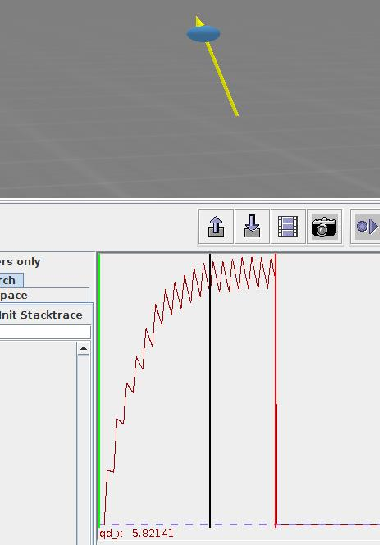
\includegraphics[scale = 0.8]{abstractRunner.pdf} 
\caption{The Abstract Runner}
\label{fig.abstractRunner}
\end{figure}

\begin{figure}[H]
\centering

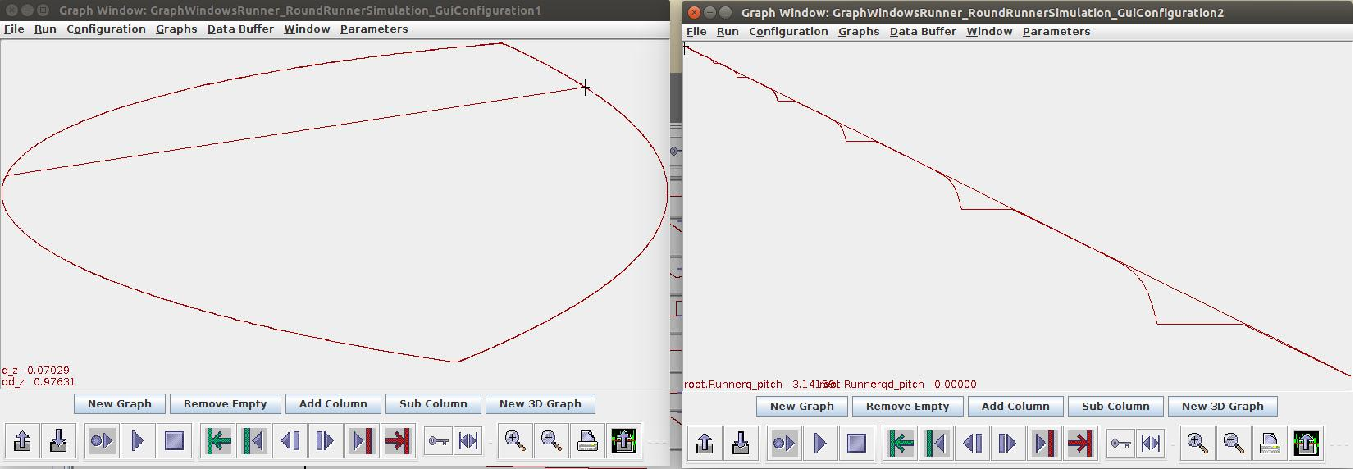
\includegraphics[scale = 0.5]{abstractRunnerPhasePortrait.pdf} 
\caption{The phase portrait of the abstract runner: phase portrait (left) of body z movement $[q\_z, qd\_z]^T$ and the pitch motion (right, the movement is converging to the origin in the upper-left corner) .}
%\label{fig.abstractRunner}
\end{figure}
\subsubsection*{Plan}
\begin{itemize}
\item Link it to the Math from Jerry's note (analysis of a linear Poincare map) to get the boundaries of stable parameters.
\end{itemize}
